\documentclass{article}
\usepackage{tikz}
\usetikzlibrary{calc, intersections, math}

\begin{document}
	\begin{figure}[h]
\centering 
	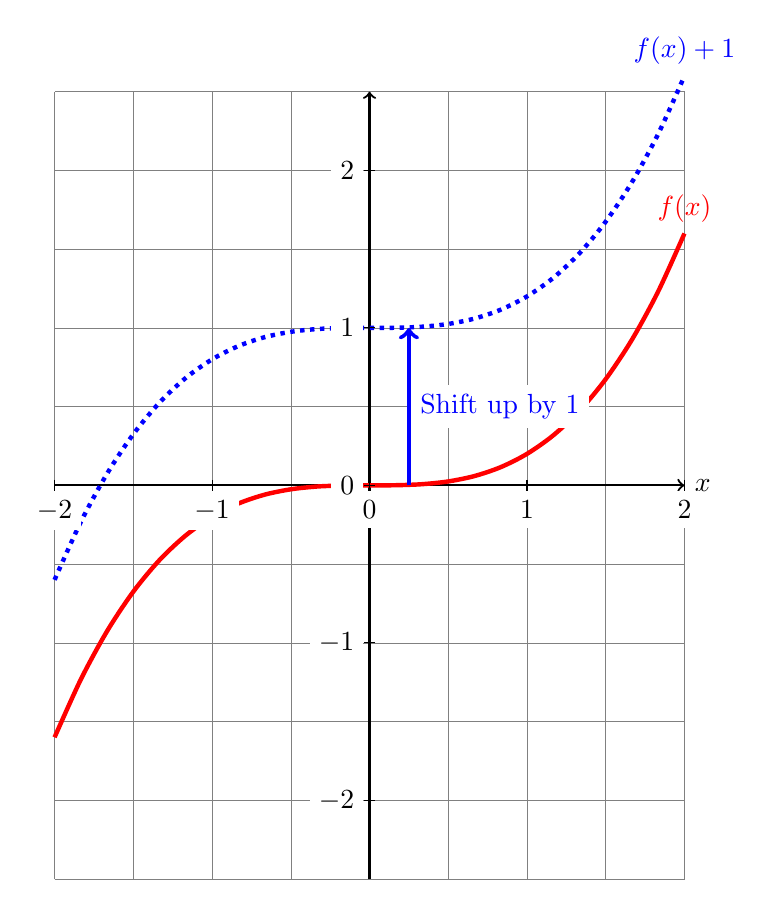
\begin{tikzpicture}[scale=2, mystyle/.style={circle,fill,scale=0.5}]

        % setting up the Cartesian Grid. Note "help lines" = "gray, very thin"
        \draw[step=.5cm,help lines] (-2,-2.5) grid (2,2.5);
        % setting up the real and imaginary axis. 
        \draw[thick, ->] (-2,0) -- (2,0) coordinate (x axis) node[right] {$x$};
        \draw[thick, ->] (0,-2.5) -- (0,2.5) coordinate (y axis);

	\draw[ultra thick,red,domain=-2:2,smooth] plot (\x,{0.2*(\x)^3}) node[above] {$f(x)$};

	\draw[ultra thick, blue, ->] (.25,0) -- (.25,1) node[midway, right, fill=white] {Shift up by $1$};

	\draw[ultra thick,blue,domain=-2:2,smooth, dotted] plot (\x,{0.2*(\x)^3+1}) node[above] {$f(x)+1$};


	\foreach \x in {-2,-1, ..., 2}
		\draw (\x cm,1pt) -- (\x cm,-1pt) node[anchor=north, fill=white] {$\x$};
 	\foreach \y in {-2,-1, ..., 2}
		\draw (1pt,\y cm) -- (-1pt,\y cm) node[anchor=east, fill=white] {$\y$};

	\end{tikzpicture}
	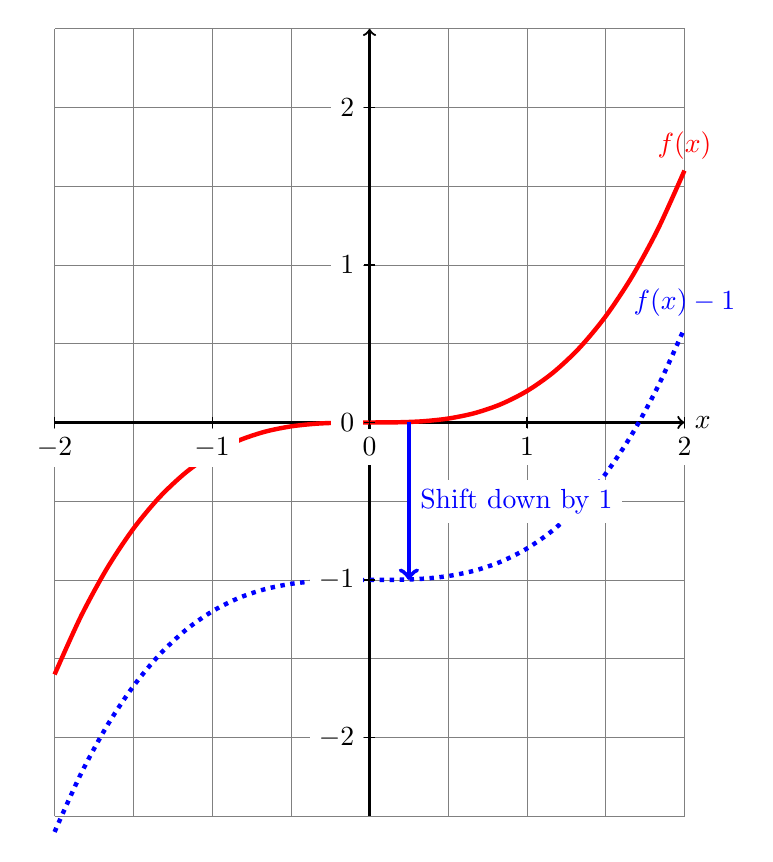
\begin{tikzpicture}[scale=2, mystyle/.style={circle,fill,scale=0.5}]

        % setting up the Cartesian Grid. Note "help lines" = "gray, very thin"
       \draw[step=.5cm,help lines] (-2,-2.5) grid (2,2.5);
        % setting up the real and imaginary axis. 
        \draw[thick, ->] (-2,0) -- (2,0) coordinate (x axis) node[right] {$x$};
        \draw[thick, ->] (0,-2.5) -- (0,2.5) coordinate (y axis);

	\draw[ultra thick,red,domain=-2:2,smooth] plot (\x,{0.2*(\x)^3}) node[above] {$f(x)$};

	\draw[ultra thick,blue,domain=-2:2,smooth, dotted] plot (\x,{0.2*(\x)^3-1}) node[above] {$f(x)-1$};

	\draw[ultra thick, blue, ->] (.25,0) -- (.25,-1) node[midway, right, fill=white] {Shift down by $1$};


	\foreach \x in {-2,-1, ..., 2}
		\draw (\x cm,1pt) -- (\x cm,-1pt) node[anchor=north, fill=white] {$\x$};
 	\foreach \y in {-2,-1, ..., 2}
		\draw (1pt,\y cm) -- (-1pt,\y cm) node[anchor=east, fill=white] {$\y$};

	\end{tikzpicture}
\caption{Left: No Interaction. Right: Interaction} \label{fig:M}
\end{figure}





	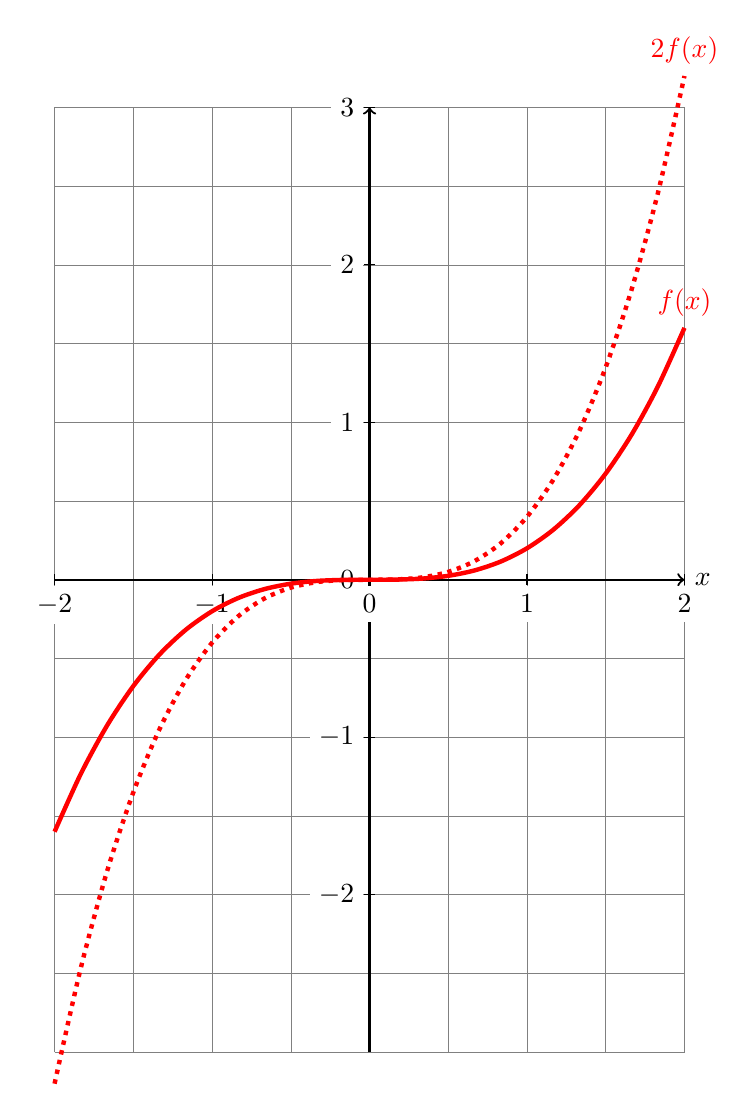
\begin{tikzpicture}[scale=2, mystyle/.style={circle,fill,scale=0.5}]

        % setting up the Cartesian Grid. Note "help lines" = "gray, very thin"
        \draw[step=.5cm,help lines] (-2,-3) grid (2,3);
        % setting up the real and imaginary axis. 
        \draw[thick, ->] (-2,0) -- (2,0) coordinate (x axis) node[right] {$x$};
        \draw[thick, ->] (0,-3) -- (0,3) coordinate (y axis);


	\foreach \x in {-2,-1, ..., 2}
		\draw (\x cm,1pt) -- (\x cm,-1pt) node[anchor=north, fill=white] {$\x$};
 	\foreach \y in {-2,-1, ..., 3}
		\draw (1pt,\y cm) -- (-1pt,\y cm) node[anchor=east, fill=white] {$\y$};

	\draw[ultra thick,red,domain=-2:2,smooth] plot (\x,{0.2*(\x)^3}) node[above] {$f(x)$};

	\draw[ultra thick,red,domain=-2:2,smooth, dotted] plot (\x,{0.4*(\x)^3}) node[above] {$2f(x)$};

	\end{tikzpicture}



\end{document}
